\documentclass[9pt]{beamer}
\usepackage{kotex}
\usepackage{amsfonts,amssymb,amsthm}
\usepackage[dvipsnames]{xcolor}
\usepackage{xcolor}
\usepackage{etoolbox}
\usepackage{braket}
\usepackage{qcircuit}

%## color
\definecolor{customBlack}{HTML}{3B4252}
\definecolor{customBlackGrey}{HTML}{434C5e}
\definecolor{cuatomGrey}{HTML}{4C566A} 
\definecolor{customWhite}{HTML}{ECEFF4} 
\definecolor{customBlue}{HTML}{6082B6}  
\definecolor{customRed}{HTML}{BF616A}
\definecolor{vividauburn}{rgb}{0.58, 0.15, 0.14}


%## Theme & custom
% \usetheme{metropolis}           % Use metropolis theme
% \metroset{block=fill}
\usetheme{moloch} % modern fork of the metropolis theme
\molochset{block=fill}
\setbeamersize{text margin left=5mm, text margin right=5mm}
\setbeamercolor{palette primary}{bg=customBlack}
\setbeamercolor{alerted text}{fg=customRed}
\setbeamercolor{itemize item}{fg=customBlue}
\setbeamercolor{enumerate item}{fg=customBlue}


%## font
\usefonttheme[onlymath]{serif}
% \setbeamerfont{normal text}{size=\small}
% \setbeamerfont{math text}{size=\tiny}


%## Theorem title, numbering
\makeatletter
\setbeamertemplate{theorem begin}
{%
\begin{\inserttheoremblockenv}
{%
\inserttheoremheadfont
\inserttheoremname
\ifx\inserttheoremaddition\@empty\else\ of\ \inserttheoremaddition\fi%
\inserttheorempunctuation
}%
}
\setbeamertemplate{theorem end}{\end{\inserttheoremblockenv}}
\makeatother
\setbeamertemplate{theorems}[numbered]  


%## Custom block
\setbeamercolor{block title}{bg=customBlue, fg=white}
\setbeamercolor{block body}{bg=customWhite, fg=customBlack}
\setbeamercolor{block title alerted}{%
    use={block title, alerted text},
    bg=customRed,
    fg=white
}
\setbeamercolor{block body alerted}{%
    use={block title, alerted text},
    bg=customWhite,
    fg=customBlack
}
\AtBeginEnvironment{definition}{%
    \setbeamercolor{block title}{fg=white,bg=customBlackGrey}
    \setbeamercolor{block body}{fg=customBlack, bg=customWhite}
}
\AtBeginEnvironment{theorem}{%
    \setbeamercolor{block title}{fg=white,bg=customBlackGrey}
    \setbeamercolor{block body}{fg=customBlack, bg=customWhite}
}
\AtBeginEnvironment{corollary}{%
    \setbeamercolor{block title}{fg=white,bg=customBlackGrey}
    \setbeamercolor{block body}{fg=customBlack, bg=customWhite}
}
\AtBeginEnvironment{lemma}{%
    \setbeamercolor{block title}{fg=white,bg=customBlackGrey}
    \setbeamercolor{block body}{fg=customBlack, bg=customWhite}
}


%! Useful command
\renewcommand{\Pr}{\text{Pr}}
% $\ast$ \underline{Proof}:
%\checkmark \underline{meaning}:

\title{2. Basic Quantum Computing with Deutsch Algorithm}
\date{\today}
\author{Vaughan Sohn}
% \institute{Centre for Modern Beamer Themes}


\begin{document}
    %#################################### 
    \maketitle
    

    %#################################### 
    \begin{frame}
        \frametitle{Contents}
        \tableofcontents
    \end{frame}

    %#################################### 
    \begin{frame}
        \frametitle{Overview of Quantum computation}
        \begin{itemize}
            \item classical computation은 initial bit-string에 logic gates를 취하여 solution을 찾는 과정을 의미한다.
            \item 이와 마찬가지로 quantum computation또한 initial \textit{qubit}-state에 \textit{quantum dynamics}를 취한 뒤, 최종 상태를 측정하여 solution을 찾는 과정이다.
            \item classical computation을 quantum에서 구현하려면 다음 사항들이 지켜져야햔다.
            \begin{itemize}
                \item state preparation이 가능해야한다.
                \item logic gate $f$를 unitary gate로 설계할 수 있어야 한다.
                \item 최종 상태를 측정한 결과가 높은 확률로 solution이어야 한다.
            \end{itemize}
        \end{itemize}
        \begin{figure}
            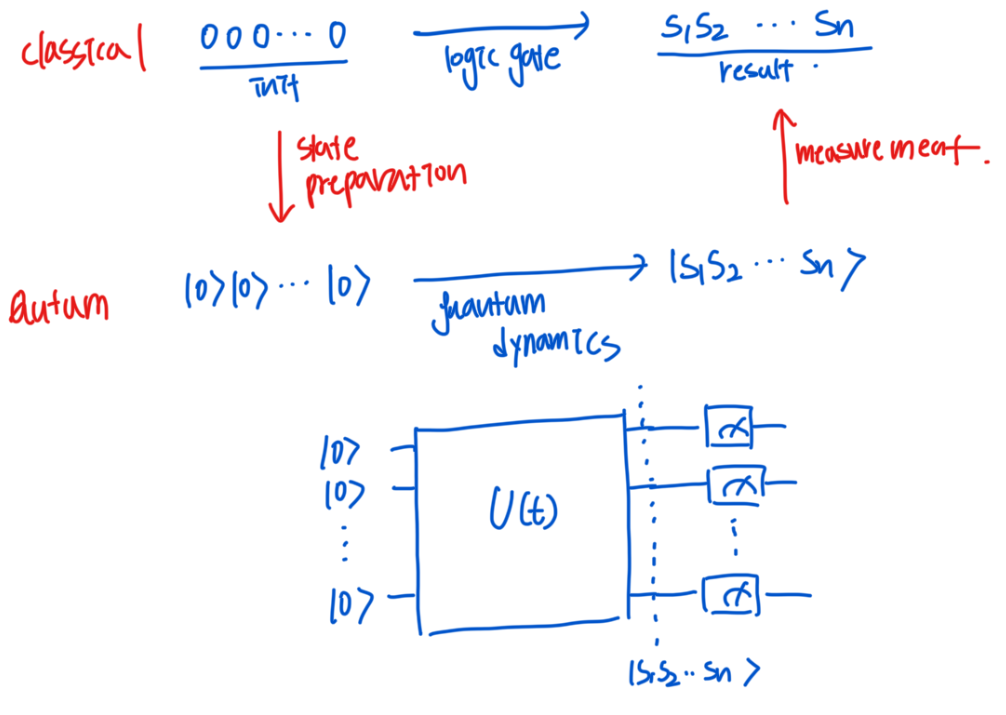
\includegraphics[width=0.55\textwidth]{image/L2_overview.png}
        \end{figure}
        \vspace{-0.3cm}
    \end{frame}

    %#################################### 
    \begin{section}{Deutsch Algorithm}
        \begin{frame}
            \frametitle{Deutsch Problem}
            \underline{Problem}: 주어진 one-but function $f: \{0, 1\} \rightarrow \{0, 1\}$이 constant인지 balance인지를 판단하는 문제
            \vspace{0.2cm}
            \begin{itemize}
                \item 가능한 4가지 함수 중에서 constant / balance function은 각각 다음과 같이 구분된다.
                \item $f(0) \oplus f(1)$의 값을 구할 수 있다면, 함수가 constant인지 아닌지를 구분할 수 있다.
                $$ \begin{cases} \text{constant} & \text{ if } f(0)\oplus f(1) = 0  \\ \text{balance} & \text{ if } f(0)\oplus f(1) = 1 \end{cases}$$
            \end{itemize}
            \begin{figure}
                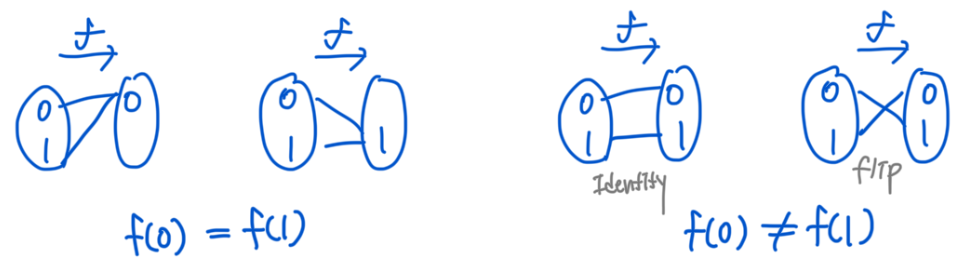
\includegraphics[width=0.6\textwidth]{image/L2_Deutsh.png}
            \end{figure}
        \end{frame}

        \begin{frame}
            \frametitle{Solutions of Deutsch Problem}
            \underline{Solutions}: 
            \vspace{0.2cm}
            \begin{itemize}
                \item classically, 주어진 함수 $f$에 대해 서로 다른 입력에 대해 \alert{2번} 호출하면 $f(0), f(1)$의 결과를 알 수 있으므로 constant인지 balance인지를 구분할 수 있다.
                \item quantumly, 다음과 같이 구성한 quantum circuit을 실행하면, $U_f$를 \alert{1번} 호출하는 것만으로 함수가 constant인지 balance인지를 구분할 수 있다. 
                \item $U_f$는 다음의 동작을 수행하는 unitary gate이다.
                $$U_f\ket x \ket y = \ket x \ket{y\oplus f(x)} $$
            \end{itemize}
            %? Deutsh
            \begin{table}[h]
                \[
                \begin{array}{c}
                \Qcircuit @C=1.1em @R=.8em {
                    \lstick{\ket{0}} & \qw    \barrier[-1.3em]{1}   &   \gate{H}   \barrier[-1.6em]{1}   & \multigate{1}{U_f}   \barrier[-1.3em]{1}   &  \gate{H}   \barrier[-1.4em]{1}   & \meter\\
                    \lstick{\ket{0}} & \gate{X} &   \gate{H} & \ghost{U_f}          & \qw       & \meter
                }
                \end{array}
                \]
            \end{table}
        \end{frame}

        \begin{frame}
            \frametitle{Deutsch Algorithm}
            앞에서 제안한 quantum circuit을 이용하면 정말로 문제를 해결할 수 있는지 확인해보자. 각각의 gate를 통과한 뒤 system의 state는 다음과 같이 변화하게 된다.
            \vspace{0.2cm}
            \begin{enumerate}
                \item $I \otimes X$
                \item $H \otimes H$
                \item $U_f$
                \vspace{1.3cm}
                \item $H \otimes I$
                \vspace{1.3cm}
            \end{enumerate}
            따라서 측정 전, 최종 상태는 다음과 같다.
            $$ (-1)^{f(0)} \frac{1}{2} \Big((\ket 0 + \ket 1) + (-1)^{f(0) \oplus f(1)}(\ket 0 - \ket 1)\Big) \ket - $$

        \end{frame}

        \begin{frame}
            \frametitle{Deutsch Algorithm}
            Deutsch Algorithm에서 얻은 최종 상태는 다음과 같다.
            $$ (-1)^{f(0)} \frac{1}{2} \Big((\ket 0 + \ket 1) + (-1)^{f(0) \oplus f(1)}(\ket 0 - \ket 1)\Big) \ket - $$

            이 상태는 $f(0) \oplus f(1)$의 값이 $0$인지 $1$인지에 따라서 다음 둘 중 하나의 상태가 된다.
            $$= \begin{cases} (-1)^{f(0)}\ket 0 \ket - & \text { if } f(0)\oplus f(1)=0\ :const \\ (-1)^{f(0)}\ket 1 \ket - & \text { if } f(0)\oplus f(1)=1\ :balanced\end{cases}$$
            
            \vspace{0.5cm}
            $\Rightarrow$ 따라서 첫번째 qubit의 값을 측정하여 $f(0)\oplus f(1)$의 값을 알아낼 수 있다.$\Box$
            
            \vspace{0.5cm}
            \begin{block}{Potential}
                Computational speedup by quantum principles may be possible!
            \end{block}
        \end{frame}
    \end{section}

    %#################################### 
    \begin{section}{Key Concept: Discrimination}
        \begin{frame}
            \frametitle{Discrimination between quantum states}
            %? State discriminate
            \underline{\textit{discrimination?}}: 서로 다른 두 상태를 완벽하게 구분할 수 있다는 의미는, \alert{동일한 POVM}으로 측정을 수행할 때 두 상태가 deterministic하게 동작해야한다는 것을 의미한다. 
            \vspace{0.2cm}
            \\Example:  
            \begin{itemize}
                \item 두 상태 $\{\ket 0, \ket 1\}$는 POVM $\{\ket 0 \bra 0, \ket 1 \bra 1\}$으로 구분할 수 있다.
                \item 두 상태 $\{\ket +, \ket -\}$는 POVM $\{\ket 0 \bra 0, \ket 1 \bra 1\}$으로 구분할 수 없다.
                \item 두 상태 $\{\ket +, \ket -\}$는 POVM $\{\ket + \bra +, \ket - \bra -\}$으로 구분할 수 있다.
            \end{itemize}
            $\Rightarrow$
            \vspace{1.8cm}
            \begin{columns}
                \begin{column}{0.5\textwidth}
                    \begin{table}[h]
                        \[
                        \begin{array}{c}
                        \Qcircuit @C=1.3em @R=.8em {
                            \lstick{\underbrace{\ket \psi}_{\{\ket 0, \ket 1\}}} & \qw   & \meter\\
                        }
                        \end{array}
                        \]
                    \end{table}
                \end{column}
                \begin{column}{0.5\textwidth}
                    \begin{table}[h]
                        \[
                        \begin{array}{c}
                        \Qcircuit @C=1.3em @R=.8em {
                            \lstick{\underbrace{\ket \psi}_{\{\ket +, \ket -\}}} & \qw   & \meter\\
                        }
                        \end{array}
                        \]
                    \end{table}
                \end{column}
            \end{columns}
        \end{frame}

        \begin{frame}
            \frametitle{Discrimination between unitaries}
            %? Unitary discriminate
            \underline{\textit{discrimination?}}: 서로 다른 두 unitary를 완벽하게 구분할 수 있다는 의미는, \alert{동일하게 준비된 state}에 각 unitary를 가한 뒤, \alert{동일한 POVM}을 측정을 수행할 때 deterministic하게 동작해야한다는 것을 의미한다.    
            \vspace{0.2cm}
            \\Example:
            \begin{itemize}
                \item $I, X$는 $\ket{\psi} = \ket{+}$, POVM $\{\ket{+}\bra +, \ket - \bra -\}$로 구분할 수 없다.
                \item $I, X$는 $\ket{\psi} = \ket{0}$, POVM $\{\ket{0}\bra 0, \ket 1 \bra 1\}$로 구분할 수 있다.
                \item $I, Z$는 $\ket{\psi} = \ket{0}$, POVM $\{\ket{0}\bra 0, \ket 1 \bra 1\}$로 구분할 수 없다.
                \item $I, Z$는 $\ket{\psi} = \ket{+}$, POVM $\{\ket{+}\bra +, \ket - \bra -\}$로 구분할 수 있다.
            \end{itemize}
            \vspace{-0.6cm}
            \begin{columns}
                \begin{column}{0.5\textwidth}
                    \begin{table}[h]
                        \[
                        \begin{array}{c}
                        \Qcircuit @C=1.3em @R=.8em {
                            \lstick{{\ket \psi}} &   \gate{\underbrace{U}_{\{I, X\}}} & \meter\\
                        }
                        \end{array}
                        \]
                    \end{table}
                \end{column}
                \begin{column}{0.5\textwidth}
                    \begin{table}[h]
                        \[
                        \begin{array}{c}
                        \Qcircuit @C=1.3em @R=.8em {
                            \lstick{{\ket \psi}} &   \gate{\underbrace{U}_{\{I, Z\}}}  & \meter\\
                        }
                        \end{array}
                        \]
                    \end{table}
                \end{column}
            \end{columns}
            \vspace{-0.3cm}
            \begin{block}{Discrimination between unitaries}
                unitary $U, V$를 완벽하게 구분하기 위해서는 다음 조건을 만족하는; 즉, 연산을 취한 뒤의 결과가 서로 \alert{orthogonal}한 $\ket \psi$를 input state로 준비해야한다.
                $$U\ket \psi\ \bot\ V \ket \psi \quad \Leftrightarrow \quad \min_\psi \braket{\psi|U^\dagger V|\psi}$$
            \end{block}
        \end{frame}

        \begin{frame}
            \frametitle{Discrimination in Deutsch Algorithm}
            \framesubtitle{Deutsch Algorithm is only Discrimination of unitaries!}
            \begin{alertblock}{Idea 1}
                Deutsch Algorithm에서 아용하는 $U_f$는 $f$에 의존하기 때문에 4가지 unitary 중에서 하나이다. 따라서 이를 구분해야한다.
                $$\Rightarrow U_f = \sum_{x,y} \ket x \bra x \otimes  \ket{{\color{red}{f(x)}}\oplus y} \bra y$$ 
            \end{alertblock}
            %? Symbols
            \begin{itemize}
                \item $U_f$가 $U_{const}, U_{balance}$중에서 어떤 unitary인지 구분하는 문제로 생각할 수 있다.
                \item 따라서 두 unitary를 구분하기 위해서는 다음의 조건을 만족하는 $\ket{\psi}$를 input으로 제공해야한다.
                  $$U_{const}\ket \psi\ \bot\ U_{balance} \ket \psi \quad \Leftrightarrow \quad \min_\psi \braket{\psi|U_{const}^\dagger U_{balance}|\psi}$$
                \item $f$의 종류에 따라 $U_{const}$는 각각 다음과 같이 설계된다.
                \begin{itemize}
                    \item $f(0) = f(1) = 0$
                    $$U_{const} = \sum_{x,y} \ket x \bra x \otimes \ket y \bra y = \boxed{I\otimes I}$$
                    \item $f(0) = f(1) = 1$
                    $$U_{const} = \sum_{x,y} \ket x \bra x \otimes \ket {1 \oplus y } \bra y = \boxed{I\otimes X}$$
                \end{itemize}
            \end{itemize}

        \end{frame}

        \begin{frame}
            \frametitle{Discrimination in Deutsch Algorithm}
            \framesubtitle{Deutsch Algorithm is only Discrimination of unitaries!}
            \begin{columns}
                \begin{column}{0.8\textwidth}
                    \begin{itemize}
                        \item $f$의 종류에 따라 $U_{balance}$는 각각 다음과 같이 설계된다.
                        \begin{itemize}
                            \item $f(0) = 0, f(1) = 1$
                            $$\begin{aligned} U_{balance} &= \ket 0 \bra 0 \otimes \sum_y \ket {y} \bra y + \ket 1 \bra 1 \otimes \sum_y \ket {1 \oplus y} \bra y 
                                \\ &= \ket 0 \bra 0  \otimes I  + \ket 1 \bra 1  \otimes X = \boxed{C(X)}\end{aligned}$$
                            \item $f(0) = 1, f(1) = 0$
                            $$\begin{aligned} U_{balance} &= \ket 0 \bra 0 \otimes \sum_y \ket {1 \oplus y} \bra y + \ket 1 \bra 1 \otimes \sum_y \ket {y} \bra y 
                                \\&= \ket 0 \bra 0  \otimes X  + \ket 1 \bra 1 \otimes I  = \boxed{(I \otimes X) C(X)}\end{aligned}$$
                        \end{itemize}
                    \end{itemize}
                \end{column}
                \begin{column}{0.2\textwidth}
                    \begin{table}[h]
                        \[
                        \begin{array}{c}
                        \Qcircuit @C=1.3em @R=.8em {
                            & \ctrl{1}  &\qw \\
                            & \targ     &\qw
                        }
                        \end{array}
                        \]
                    \end{table}
                    \begin{table}[h]
                        \[
                        \begin{array}{c}
                        \Qcircuit @C=1.3em @R=.8em {
                            & \ctrlo{1}  &\qw \\
                            & \targ     &\qw
                        }
                        \end{array}
                        \]
                    \end{table}
                \end{column}q
            \end{columns}
            \vspace{0.4cm}
            \begin{itemize}
                \item $U_{const}$는 single gate $I, X$만을 이용하여 구현할 수 있지만, $U_{balance}$는 two-qubit gate인 $C(X)$을 사용해야한다.
                \item Deutsch problem은 unitary operator $U_f$가 \textit{local unitary}인지 \textit{entangling unitary}인지를 구분하는 문제이다!
            \end{itemize}
        \end{frame}
    \end{section}

    %#################################### 
    \begin{section}{Key Concept: Phase estimation}
        \begin{frame}
            \frametitle{Phase estimation: preparation}
            \begin{block}{Goal}
                Phase estimation의 목적은, 어떤 unitary operator $U$가 가해진 결과로서 만들어진 phase $\varphi$를 추정하는 것이다. ($\varphi$는 모른다고 가정한다.)
                $$ U \ket{\psi} = e^{i2\pi \varphi} \ket \psi \Rightarrow \varphi.$$
            \end{block}
            \begin{itemize}
                \item (아이디어 1) $\ket u$는 unitary operator $U$의 eigenvector이며, 다음을 만족한다.
                $$U\ket{u} = \lambda \ket{u} = e^{i 2\pi \varphi} \ket{u}$$
                \item $U^{2^k}$ gate는 $U$를 $2^k$번 적용하는 gate이므로 다음과 같이 표현된다.
                $$ U^{2^k} = (e^{i 2\pi \varphi})^{2^k} \ket u = e^{i 2^{k+1}\pi \varphi}\ket u$$
                \item $C(U^{2^k})$ gate를 superposition state $\ket +\ket{u}$에 가하면, 다음을 얻게 될 것이다.
                $$(I \otimes U^{2^k}) \frac{1}{\sqrt 2}(\ket 0 \ket u+ \ket 1 \ket u)  = \frac{1}{\sqrt 2}(\ket 0 \ket u + e^{i2\pi (2^{k}\varphi)}\ket 1 \ket u)$$
                $$\boxed{\frac{1}{\sqrt 2}( \ket 0 + e^{i2\pi (2^{k}\varphi)}\ket 1 )\otimes \ket u}$$
            \end{itemize}
            %? General Deutsh (first step)

        \end{frame}

        \begin{frame}
            \frametitle{Phase estimation: preparation}
            
            따라서 $\ket{0^{\otimes t}}$에 $H^{\otimes t}$ gate를 취하여 중첩상태 $\ket{+^{\otimes t}}$가 되도록 하면, $C(U^{2^k})$를 적용한 결과로 다음과 같은 최종상태를 얻게 된다.
            \small \[ \begin{aligned} &\frac{1}{(\sqrt 2)^t}\left[ \Big(\ket 0 + e^{i 2\pi (2^{t-1}\varphi)}\ket 1\Big) \Big(\ket 0 + e^{i 2 \pi  ({2^{t-2}\varphi})}\ket 1\Big) \cdots \Big(\ket 0 + e^{i 2\pi ({2^{0}\varphi})}\ket 1 \Big)\right] 
                \\ &= \frac{1}{(\sqrt 2)^t}\Big[ \ket{0 \cdots 00} +e^{i2\pi(2^0\varphi)}\ket{0\cdots 01} + e^{i2\pi(2^1\varphi)}\ket{0\cdots 10} + e^{i2\pi(2^1+2^{0})\varphi}\ket{0\cdots 11}
                \\ &\qquad + \cdots + {\color{red}e^{i2\pi (2^{t-1}+2^{t-2}+\cdots +2^0)\varphi} }\ket{1 \cdots 11}\Big] = \boxed{\frac{1}{(\sqrt {2})^t} \sum^{2^t-1}_{\ell=0} e^{i2\pi \varphi \cdot \ell} \ket{\ell}} \end{aligned} 
            \]
            \vspace{-0.2cm}

            \textit{where} $\ket \ell = \ket{\ell_{t-1} 2^{t-1} + \cdots + \ell_0 2^0}$
            
            \begin{figure}
                \centering
                \Qcircuit @C=1.2em @R=0.9em {
                    & & & &\lstick{\ket 0} &\gate{H} &\qw \barrier[-1.8em]{6}&\qw                      &\qw                    &\qw & \dots &       &\ctrl{6}                   &\rstick{\frac{1}{\sqrt 2}(\ket 0 + e^{2\pi i \varphi 2^{t-1}}\ket 1)}\qw\\
                    & & & &                &\vdots   &                       &                       &                       &    & \dots &       &                           &           \\
                    & & & &\lstick{\ket 0} &\gate{H} &\qw                    &\qw                    &\ctrl{4}               &\qw & \dots &       &\qw                        &\rstick{\frac{1}{\sqrt 2}(\ket 0 + e^{2\pi i \varphi 2^{2}}\ket 1)}\qw        \\
                    & & & &\lstick{\ket 0} &\gate{H} &\qw                    &\ctrl{3}               &\qw                    &\qw & \dots &       &\qw                        &\rstick{\frac{1}{\sqrt 2}(\ket 0 + e^{2\pi i \varphi 2^{1}}\ket 1)}\qw        \\
                    & & & &\lstick{\ket 0} &\gate{H} &\ctrl{2}               &\qw                    &\qw                    &\qw & \dots &       &\qw                        &\rstick{\frac{1}{\sqrt 2}(\ket 0 + e^{2\pi i \varphi 2^{0}}\ket 1)}\qw        \\
                    & & & &                &         &                       &                       &                       &    &       &       &                           &                                                                              \\
                    & & & &\lstick{\ket u} &{/}\qw   &\gate{U^{2^0}}         &\gate{U^{2^1}}         &\gate{U^{2^2}}         &\qw & \dots &       &\gate{U^{2^{t-1}}}         &\rstick{\ket u}\qw
                }
            \end{figure}
            \vspace{-0.5cm}
        \end{frame}

        \begin{frame}
            \frametitle{Quantum Fourier Transform}
            \begin{alertblock}{Idea of phase estimation}
                (아이디어 2) 일련의 준비과정으로 얻은 최종 상태에 \textit{Inverse Quantum Fourier Transform}을 가하면, phase $\varphi$를 얻을 수 있다!
            \end{alertblock}

            \vspace{0.2cm}
            \begin{theorem}[Classical fourier transform]
                time-domain data를 frequency domain data로 변환하는 classical fourier transform은 다음과 같이 정의된다.
                $$ x_k \overset{DFT}{\rightarrow} y_k \triangleq \frac{1}{\sqrt N} \sum^{N-1}_{j=0} e^{{i(2\pi/N)} jk}x_j$$
            \end{theorem}
            \vspace{0.2cm}
            \begin{theorem}[Quantum fourier transform]
                이를 basis $\{\ket k\}$를 다른 basis $\{\ket j\}$에 대한 linear combination으로 변환하는 quantum fourier transform으로 생각할 수 있다.
            $$\ket k \overset{U_{\mathcal F}}{\rightarrow}  \ket{\tilde k}  \triangleq \frac{1}{\sqrt N} \sum^{N-1}_{j=0} e^{\frac{i2\pi}{N} jk} \ket j $$
            \end{theorem}\label{thr:qft}
            
        \end{frame}

        \begin{frame}
            \frametitle{Quantum Fourier Transform}
            \begin{itemize}
                \item 따라서 QFT를 이용하면 basis $\{\ket k\}$에 대해 표현된 어떤 임의의 state $\ket x$를 다른 basis $\{\ket j\}$에 대한 linear combination으로 변환할 수 있다.
                $$\ket x \rightarrow \sum_k x_k \frac{1}{\sqrt N} \sum^{N-1}_{j=0} e^{\frac{i2\pi}{N} jk} \ket j \triangleq  \sum_j y_j \ket j $$
                where $\ket x$ is
                $$\ket x = \sum_k x_k \ket{k}.$$
                \item Quantum Fourier Transform을 수행하는 gate는 다음과 같다.
                $$U_\mathcal F = \sum_k \ket{\tilde k} \bra{k}, \qquad U_{\mathcal F}^\dagger = U_{\mathcal F^{-1}}= \sum_{k'} \ket{ {k'}} \bra{\tilde {k'}}$$

                이렇게 정의되는 gate는 unitary ($\ast$)이기 때문에, valid quantum gate이다. 
                \\$\Rightarrow$
                \vspace{1cm}
                $$ U_{\mathcal F^{-1}}U_{\mathcal F} \ket{\psi} = \ket{\psi}$$
            \end{itemize}
        \end{frame}

        \begin{frame}
            \frametitle{Quantum Fourier Transform}
            \begin{itemize}
                \item 앞에서 정의한 \textit{inverse} quantum fourier transform $U_{F^{-1}}$은 다음과 같이 동작한다.
                $$\ket{\tilde k}  \triangleq \frac{1}{\sqrt N} \sum^{N-1}_{j=0} e^{\frac{i2\pi}{N} j {\color{red}k}} \ket j \overset{U_{\mathcal F ^{-1}}}{\rightarrow} \ket k $$
                where
                $$ U_{\mathcal F}^\dagger = U_{\mathcal F^{-1}}= \sum_k \ket{ k} \bra{\tilde k}$$
                \item 어떤 superposition quantum state가 각 항마다 중복되는 phase term $k$를 가지고 있는 경우, IQFT는 그 값을 구해내는데 사용할 수 있다.
                \item Phase estimation의 전체 과정은 다음과 같다.
                \begin{table}[h]
                    \[
                    \begin{array}{c}
                    \Qcircuit @C=1.3em @R=.8em {
                        \lstick{\ket {0^{\otimes t}}}  &{/}\qw &\gate{H^{\otimes t}}&\ctrl{1}   &\gate{QFT^\dagger} &\meter & \varphi\\
                        \lstick{\ket u}                &{/}\qw &\qw                 &\gate{U^j} &\qw                &\rstick{\ket u}\qw
                    }
                    \end{array}
                    \]
                \end{table}
            \end{itemize}
            \vspace{0.4cm}
            $\Rightarrow$ 따라서 phase estimation preparation 상태가 가지는 중복되는 phase term $\varphi$를 IQFT를 사용하여 구할 수 있다!
        \end{frame}

        \begin{frame}
            \frametitle{Phase estimation in Deutsch Algotirhm}
            \framesubtitle{Deutsch Algorithm requires Phase Estimation to get the superposition result!}
            \begin{itemize}
                \item $N=2^t$라고 두면 최종상태는 다음과 같이 표현되며 이는 $\ket{N \varphi}$에 대해 QFT를 수행한 결과로 생각해볼 수 있다.
                $$ \frac{1}{(\sqrt {2})^t} \sum^{2^t-1}_{\ell=0} e^{i2\pi \varphi \cdot \ell} \ket{\ell} = \frac{1}{\sqrt N} \sum^{N-1}_{\ell=0} e^{\frac{i2\pi}{N} {\color{red}(N\varphi)} \cdot \ell} \ket \ell$$ 
                \item 따라서 이 상태에 대해 IQFT를 취하면 phase term을 얻을 수 있다.
                $$U_{\mathcal F^{-1}}\left( \frac{1}{\sqrt N} \sum^{N-1}_{\ell=0} e^{\frac{i2\pi}{N} {(N\varphi)} \cdot \ell} \ket \ell \right) = \boxed{\ket{N\ell}}$$
                \item Deutsch algorithm은 phase estimation에서 다음을 만족하는 특수한 경우이다.
                \begin{itemize}
                    \item $t=1$
                    \item $U_f$의 eigenvector인 $\ket -$로 초기화한다. ($\ket +$는 phase가 0이된다.)
                    \item 이때 $U_f$는 첫 번째 qubit의 값에 따라서 연산하는 controlled unitary로 생각할 수 있다.
                    \item $t=1$이므로 IQFT역시 $H$ gate 하나로 쉽게 구현할 수 있다.
                \end{itemize}
                    
            \end{itemize}

        \end{frame}
    \end{section}

    %#################################### 
    \begin{section}{Universal gate set}
        \begin{frame}
            \frametitle{Univerial gate set}
            \begin{itemize}
                \item Classical computer에서는 NAND나 NOR만 사용하여 모든 computation을 수행할 수 있다.
                \item 이처럼 quantum computer에서도 모든 gate가 아니라 일부의 gate들만 사용하여 모든 computation을 수행할 수 있는 \textit{universal gate set}이 존재한다.
                \item 일반적으로 다음 3가지 종류를 많이 사용한다.
                \begin{itemize}
                    \item $\{C(X), \text{ all single-qubit gates}\}$
                    \item $\{C(X), H, T\}$ (in our class)
                    \item $\{C^2(X), H\}$
                \end{itemize}
                \item all single-qubit gates는 \textit{infinite}하기 때문에 이를 continuous gate set이라고 말하며, 노이즈의 영향을 많이 받게된다.
                \item 반면 다른 gate set들은 각각 3개, 4개의 finite한 gate 종류만 사용하기 때문에 discrete gate set이라고 부른다. 
            \end{itemize}
        \end{frame}

        \begin{frame}
            \frametitle{Prerequisite: bloch sphere and rotation gate}
            \textbf{Bloch sphere}
            \\single qubit의 state는 3차원의 구에서 2개의 parameter $(\theta, \phi)$로 표현할 수 있다.
            $$ \ket{\psi(\theta, \phi)} = \cos \frac{\theta}{2} \ket 0 + e^{i \phi} \sin  \frac{\theta}{2}  \ket 1 $$ 
            $$ \longrightarrow \vec{\psi} = (\sin \theta \cos \phi,\ \sin \theta \sin \phi, \ \cos \theta)$$
            \begin{figure}
                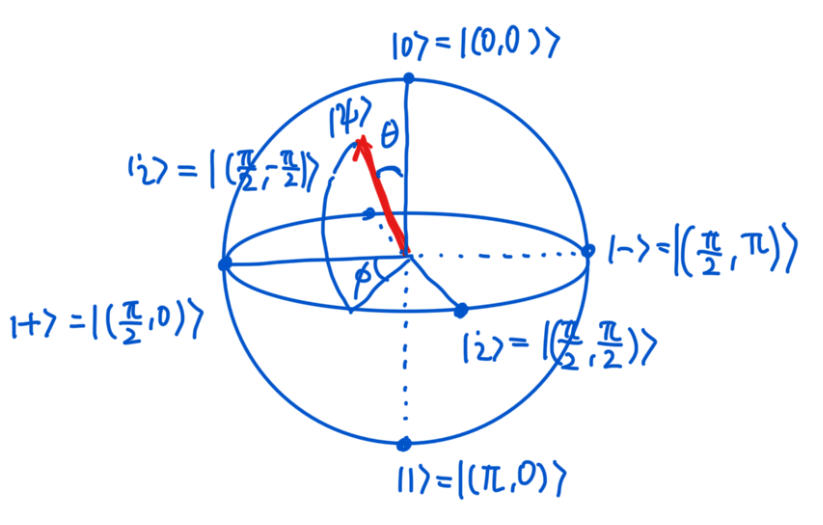
\includegraphics[width=0.5\textwidth]{image/L2_bloch_sphere.png}
            \end{figure}
        \end{frame}

        \begin{frame}
            \frametitle{Prerequisite: bloch sphere and rotation gate}
            \textbf{Rotation gate}
            \\Bloch sphere에서 특정 축 $\hat n$을 기준으로 $\alpha$만큼 회전하는 연산을 rotation gate라고 하며, 다음과 같이 정의할 수 있다.
            $$\begin{aligned} R_{\hat n}(\alpha) &= e^{-i \alpha/2 (\hat n \cdot \vec \sigma)} =  e^{-i \alpha/2 (n_x X + n_y Y + n_z Z)} \\ &= \sum^\infty_{n=0} \frac{1}{n!} (-i \frac{\alpha}{2})^n (\hat n \cdot  \vec\sigma)^n \end{aligned}$$
            \begin{itemize}
                \item Example: $Z$-axis rotation gate
                \\ 예를 들어, $\hat n = (0, 0, 1)$이라면 다음과 같은 rotation gate를 얻게된다. ($\ast$)
                $$\begin{aligned} R_{Z}(\alpha) &= \sum^\infty_{n=0} \frac{1}{n!} \left( -i \frac{\alpha}{2} \right)^n (Z)^n = \begin{pmatrix} e^{-i\alpha/2} & 0 \\ 0 &  e^{i\alpha/2}  \end{pmatrix} \end{aligned}$$
                즉, 이 gate는 $Z$축을 기준으로 $\alpha$만큼 회전하는 연산을 수행한다.    
            \end{itemize}
            \begin{columns}
                \begin{column}{0.7\textwidth}
                    \small \[ \begin{aligned} R_{Z}(\alpha) \ket{\psi(\theta, \phi)} &= \begin{pmatrix} e^{-i\alpha/2} & 0 \\ 0 &  e^{i\alpha/2}  \end{pmatrix}  \begin{pmatrix} \cos \frac{\theta}{2}  \\  e^{i \phi} \sin \frac{\theta}{2} \end{pmatrix} \\  &= e^{-i \alpha/2}\left[ \cos \frac{\theta}{2} \ket 0 + e^{i(\alpha+\phi) } \sin \frac{\theta}{2}  \ket 1 \right]  \\ &= \ket{\psi(\theta, \phi {\color{red}+\alpha})}\end{aligned} 
                    \]
                \end{column}
                \begin{column}{0.3\textwidth}
                    \begin{figure}
                        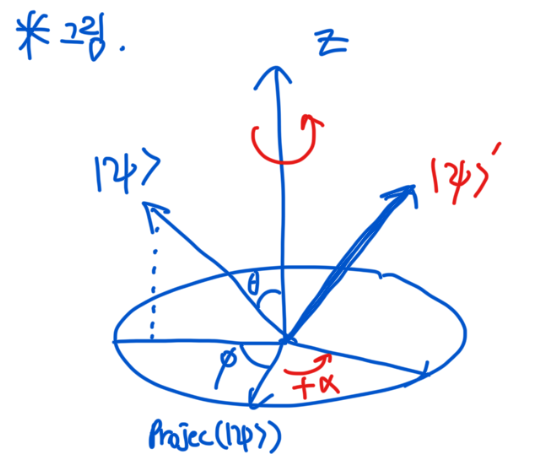
\includegraphics[width=0.9\textwidth]{image/L2_rotation.png}
                    \end{figure}                    
                \end{column}
            \end{columns}

        \end{frame}

        \begin{frame}
            \frametitle{Prerequisite: bloch sphere and rotation gate}
            \begin{itemize}
                \item Example: $Y$-axis rotation gate
                \\ 반면, $\hat{n} = (0, 1, 0)$이라면 다음과 같은 rotation gate를 얻게된다. ($\ast$)
                $$\begin{aligned} R_Y (\alpha) &= \left( \cos \frac{\alpha}{2} \right) I - i \left( \sin \frac{\alpha}{2} \right)  Y  = \begin{pmatrix} \cos \frac{\alpha}{2} & -\sin \frac{\alpha}{2} \\  \sin \frac{\alpha}{2} & \cos \frac{\alpha}{2} \end{pmatrix} \end{aligned}$$
                특히, $\alpha = \pi/2$일 떄, $R_{Y}(\pi/2)$는 Hadamard gate와 동일하다.
                $$R_Y\left( \frac{\pi}{2} \right) \ket 0 = \begin{pmatrix} \frac{1}{\sqrt 2} & - \frac{1}{\sqrt 2} \\ \frac{1}{\sqrt 2} & \frac{1}{\sqrt 2} \end{pmatrix} \begin{pmatrix} 1 \\ 0\end{pmatrix} = \ket +$$
                \item $X$ gate를 이용하면 회전 방향을 바꾸는 효과를 얻을 수 있다.
                \begin{itemize}
                    \item $XR_Y(\theta)X = R_Y(-\theta)$
                    \item $XR_Z(\theta)X = R_Z(-\theta)$
                \end{itemize}
            \end{itemize}
        \end{frame}

        \begin{frame}
            \frametitle{Controlled unitary decomposition}
            \begin{itemize}
                \item 앞에서 우리는 Deutsch algorithm이 phase estimation의 특수한 경우임을 알았고, phase estimation을 위한 quantum circuit의 구조까지 배웠다.
                \item 그렇다면, phase estimation circuit을 이루는 \textit{controlled unitary}를 universal gate만을 사용하여 구현하려면 어떻게 해야할까?
                \item controlled unitary는 다음과 같이 표현할 수 있다.
                \item 다음의 정리를 이용하면, controlled unitary를 $\{C(X), \text{ all single-qubit gates}\}$ gate set으로 표현할 수 있다!
            \end{itemize}
            \vspace{0.2cm}
            \begin{theorem}[Decomposition of unitary]
                Arbitrary single-qubit gate $U$는 다음의 행렬로 decomposition할 수 있다.
                $$U = R_Z(-\alpha) R_Y(-\theta) R_Z(-\beta)$$
                by matrix representation,
                $$U = \begin{pmatrix} e^{i \alpha/2} & 0 \\ 0 & e^{- i \alpha/2} \end{pmatrix} \begin{pmatrix}  \cos \frac{\theta}{2} & \sin \frac{\theta}{2} \\ -\sin \frac{\theta}{2} & \cos \frac{\theta}{2} \end{pmatrix}  \begin{pmatrix} e^{i \beta/2} & 0 \\ 0 & e^{- i \beta/2}  \end{pmatrix} $$
            \end{theorem}
            
        \end{frame}

        \begin{frame}
            \frametitle{Example: Controlled Y-axis rotation gate}
            Example: Controlled Y-axis rotation gate를 다음과 같이 decomposition할 수 있음을 보이자.
            $$ \ket{0}\bra 0 \otimes I + \ket 1 \bra 1 \otimes R_Y(\theta) = (C(X)){(I\otimes R_Y(-\theta/2)){(C(X))(I\otimes R_Y(\theta/2))}} $$
            %?universial
            \vspace{-1cm}
            \begin{columns}
                \begin{column}{0.35\textwidth}
                    \begin{table}[h]
                        \[
                        \begin{array}{c}
                        \Qcircuit @C=1.3em @R=.9em {
                            & \ctrl{1} &\qw \\
                            & \gate{R_Y(\theta)} &\qw
                        }
                        \end{array}
                        \]
                    \end{table}
                \end{column}
                $=$
                \begin{column}{0.65\textwidth}
                    \begin{table}[h]
                        \[
                        \begin{array}{c}
                        \Qcircuit @C=1.3em @R=.9em {
                            & \qw                  &\ctrl{1}   &\qw                     &\ctrl{1} &\qw &\qw\\
                            & \gate{R_Y(\theta/2)} &\targ      &\gate{R_Y(-\theta/2)}   &\targ    &\gate{I} & \qw
                        }
                        \end{array}
                        \]
                    \end{table}                
                \end{column}
            \end{columns}
            \begin{lemma}
                (hint:) 다음의 lemma를 활용하라.
                $$ Xe^{i \phi Y} = e^{-i \phi Y} X,\quad X R_Y(-2\phi)= R_Y(2\phi) X $$ 
            \end{lemma}
            $\Rightarrow$
            \vspace{1.5cm}
        \end{frame}

        \begin{frame}
            \frametitle{Approximating quantum circuits via discrete gate set}
            \framesubtitle{Solovay-Kitaev Theorem}
            \begin{theorem}[Solovay-Kitaev Theorem]
                모든 arbitrary unitary gate에 대해서, 그 error가 매우 작은 값으로 bound되도록 근사시킨 gate $W$가 존재하며, $W$는 discrete gate set의 gate들로만 이루어진다.
                $$\forall U,\ \exists W \in G^l = \{g_1g_2 \cdots g_l\ : \ g_i \in G = \{H, T, C(X)\} $$
                $$s.t., \quad |U-W| < \epsilon $$
            \end{theorem}
            \vspace{0.2cm}
            $\ast$ \underline{Proof}:
            \begin{itemize}
                \item (아이디어) 모든 single-qubit gate는 rotation gate들의 product로 이루어지므로, discrete gate set을 사용하여 서로다른 축에 대한 rotation gate를 구현하자.
                \item $THTH$로 새로운 축 $\hat n$에 대해 $\hat \theta$만큼 회전하는 rotation gate를 구현할 수 있다.
                $$\begin{aligned} THTH &=  e^{-i\frac{\pi}{8}Z}e^{-i\frac{\pi}{8}X} = \\ &= \boxed{\cos ^2 \frac{\pi}{8} I-i\left[\cos \frac{\pi}{8}(X+Z)+\sin \frac{\pi}{8} Y\right] \sin \frac{\pi}{8}} \end{aligned}$$
            \end{itemize}
        \end{frame}

        \begin{frame}
            \frametitle{Approximating quantum circuits via discrete gate set}
            \framesubtitle{Solovay-Kitaev Theorem}
            $\ast$ \underline{Proof}: (contd.)
            \begin{itemize}
                \item $H$ gate를 이용하면 다른 축 $\hat m$에 대한 rotation gate도 만들 수 있다.
                \item $THTH$로 새로운 축 $\hat n$에 대해 $\hat \theta$만큼 회전하는 rotation gate를 구현할 수 있다.
                $$R_{\hat m} (\hat \theta) \triangleq H R_{\hat n} (\hat \theta) H $$
                \item (아이디어) Kronecker approximation theorem을 이용하면 어떤 충분히 큰 $N$에 대해서, $R_{\hat n}(\hat \theta)$를 $N$번 곱하면 $R_{\hat n} (\theta)$를 어떤 $\theta\ (\theta \in [0, 2\pi))$에 대해서도 충분히 작은 error-rate로 근사할 수 있다.
                $$\left \{R_{\hat n} \left( \hat \theta \right) \right\}^N \approx R_{\hat n} (\varphi)$$
                \item 따라서 single qubit gate가 다음과 같이 decomposition될 때,
                $$U = e^{i\varphi} R_{\hat n}(\alpha) R_{\hat m}(\beta) R_{\hat n}(\gamma)$$
                universal gate set $\{H, T, CNOT\}$을 사용하여 다음과 같이 근사할 수 있다.$\Box$
                $$U \approx e^{i\varphi}(THTH)^{N_1}(H(THTH)H)^{N_2}(THTH)^{N_3}$$
                
            \end{itemize}
        \end{frame}

    \end{section}


    %#################################### 
    \begin{frame}{References}
        
        \begin{itemize}
            \item Lecture notes for EE547: Introduction to Quantum Information Processing (Fall 2024)
        \end{itemize}
        \vspace{6cm}
    \end{frame}

\end{document}